\documentclass[UTF8,openany]{ctexbook}
\usepackage{amsmath}
\usepackage{amssymb}
\usepackage{tikz}
\usepackage[european]{circuitikz}
\begin{document}
    
    \chapter{非线性电阻电路}

    \section{非线性电阻电路的基本分析方法}
    \subsection{图解法}
    \par 图解法是相对较为直观的方法,它不能求出精确的解,但是可以分析大致的特征。对于含有非线性电阻的电路,
    可以将其拆分为两个对接的网络,一方是线性网络,一方是非线性网络,并且用关联参考方向、源关联参考方向定义
    两个网络。作出两个网络的伏安特性曲线,其交点就是所求的解。这个解是粗略的,下面的方法更能求得精确的或者
    接近精确值的解。
    \subsection{牛顿-拉夫逊迭代法}
    \par 在上面图解法的基础上,牛顿-拉夫逊迭代法可以求得尽可能精确的解。联立曲线方程,得到一个方程
    $f(x)=0$。这个方程是超越的,那么可以用迭代法。给定一个大致的解$x^{(0)}$,每一次迭代(这里是$k+1$次)都对上一次的解
    进行一个修正$\Delta x^{(k)}$,也就是$x^{(k+1)}=x^{(k)}+\Delta x^{(k)}$。由Taylor展开可以得到
    \[
    f(x^{(k+1)})=f(x^{(k)}+\Delta x^{(k)})\approx f(x^{(k)})+f'(x^{(k)})\Delta x^{(k)}=0    
    \]
    \[
    \Delta x^{(k)}=-\frac{f(x^{(k)})}{f'(x^{(k)})}    
    \]
    \[
    x^{(k+1)}=x^{(k)}-\frac{f(x^{(k)})}{f'(x^{(k)})}  
    \]
    \par 设定一个精确度$\varepsilon$,如果$f(x^{(k)})<\varepsilon$,就认为精度足够了,迭代终止。一般而言,不到十次就可以得到比较精确的解。
    这种方法适用于计算机分析,手工分析更常用后面的方法。
    \subsection{分段折线法}
    \par 分段折线法是一种化曲为直的方法。如果伏安特性曲线有明显的分区特性,就可以用直线代替曲线,从而手工解出较为准确的解。对于曲线
    的一部分,可以利用割线或者切线来代替曲线。有时不知道位于哪个工作区时,可以先假设位于其中某个区,然后计算验证,
    如果符合,则假设成立;如果不符合,应该另外设别的区。分段折线法更多地会结合下面的方法运用。
    \subsection{局部线性法}
    \par 局部线性法适用于直流与交流叠加的电压:$v=V_0+\Delta v$,习惯用大写字母表示直流量,小写字母表示交流量。对于含有此类电信号的非线性电路,
    采取的方法是将直流和交流分别分析:首先只看直流,利用前面提到的方法确定直流工作点(区);然后只看交流,确定更细致的关系。对于电源、电阻、电容、
    电感元件,在直流情形和交流情形的分析如下:
    \par (1)电源:将电源分为恒压源和交流电压源,在直流情形下,将交流电压源短路即可;在交流情形下,将恒压源短路即可。
    \par (2)电阻:对于线性电阻,直流情形和交流情形的分析相同;对于非线性电阻,其伏安特性曲线并非直线,在直流情形下按照前面的方法分析,在交流情形下
    视为电阻,其阻值是伏安特性曲线在直流工作点切线斜率的导数,这个电阻称为\textbf{微分电阻}。
    \begin{center}
        \begin{tikzpicture}
            \draw[-stealth] (-1,0) to (3,0) node[right] {$v$};
            \draw[-stealth] (0,-1) to (0,3) node[above] {$i$};
            \draw (0,0) parabola (2,4);
            \draw[blue] (0,-1) to (2,3);
        \end{tikzpicture}
    \end{center}
    \par (3)电容电感:以电容为例,其电压电流特性为
    \[
    i(t)=C\frac{\mathrm{d}v(t)}{\mathrm{d}t}    
    \]
    \par 我们设$v(t)=V_0+V_m\cos\omega t$,则可以得到$i(t)=-\omega C V_m\sin\omega t$,因而
    \[
    \frac{(v(t)-V_0)^2}{V_m^2}+\frac{i(t)^2}{\omega^2C^2V_m^2}=1    
    \]
    \par 当$V_0=0$时,其图像是以原点为中心的椭圆,长半轴为$\omega CV_m$,短半轴为$V_m$。对于高频交流电压,
    其长半轴将是无限长,此时近似为经过原点且垂直于$v$轴的直线,也就是短路。而当$\omega=0$时,则相当于开路。当$V_0\neq 0$时,则抽象为恒压源。
    \begin{center}
        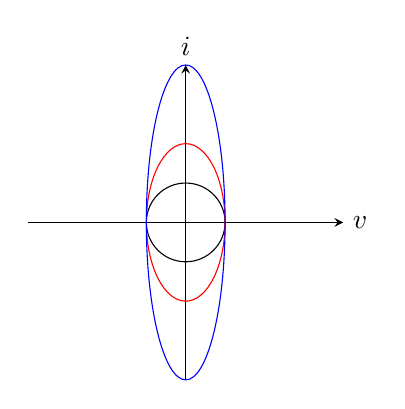
\begin{tikzpicture}
            \draw[-stealth] (-2,0) to (2,0) node[right] {$v$};
            \draw[-stealth] (0,-2) to (0,2) node[above] {$i$};
            \draw (0,0) circle (0.5);
            \draw[red] (0,0) circle (0.5 and 1);
            \draw[blue] (0,0) circle (0.5 and 2);
        \end{tikzpicture}
    \end{center}
    \par 同理,对于电感元件,当初始电流为0时,对于高频交流电压相当于开路,对于直流电压则相当于短路。
    \par 综合上述几方面,我们可以得到直流与交流分析时的元件处理办法。
    \begin{center}
    \begin{tabular}{|c|c|c|}
        \hline
        \bfseries 元件 & \bfseries 直流分析 & \bfseries 交流分析 \\
        \hline
        直流源 & 不变 & 屏蔽 \\
        \hline
        交流源 & 屏蔽 & 不变 \\
        \hline
        电阻 & 不变 & 微分电阻替代 \\
        \hline
        耦合电容 & 开路 & 短路 \\
        \hline
        高频扼流圈 & 短路 & 开路 \\
        \hline
    \end{tabular}
    \end{center}
    \par 考虑单端口线性网络(L)与非线性网络(N)的对接,假设非线性网络的GOL为$v=f(i)$,则有
    \[
    v_{TH}-Ri=f(i)    
    \]
    \par 现在假设电源电压是波动的,我们有$v_{TH}=V_{TH}+\Delta v$,$i=I_0+\Delta i$,则上述方程可以拆解为
    \begin{align*}
        V_{TH}-RI_0=f(I_0)\\
        \Delta v-r\Delta i=f'(I_0)\Delta i
    \end{align*}
    \par 如果网络L是阻性的,则$R=r$;如果含有耦合电容或高频扼流圈,则会出现$R\neq r$,需要分别处理。
    \par 现在考虑二端口网络。假设有两个二端口网络连接在一起,则需要从四种连接方式中选取较为合适的。以\textbf{\textit{z}}
    参量为例,对于线性网络,我们有
    \[
    \begin{pmatrix}
        v_{L1} \\ v_{L2}
    \end{pmatrix}
    =
    \begin{pmatrix}
        Z_{11} & Z_{12} \\ Z_{21} & Z_{22}
    \end{pmatrix}
    \begin{pmatrix}
        i_{L1} \\ i_{L2}
    \end{pmatrix}
    +
    \begin{pmatrix}
        v_{TH1} \\ v_{TH2}
    \end{pmatrix}
    \]
    \par 对于非线性网络,我们有
    \[
    \begin{pmatrix}
        v_{N1} \\ v_{N2}
    \end{pmatrix}
    =
    \begin{pmatrix}
        f_1(i_{N1},i_{N2})\\
        f_2(i_{N1},i_{N2})
    \end{pmatrix}    
    \]
    \par 两个网络串串连接,之后两个端口短路处理(电路是闭合的),那么我们可以得到
    \[
    \begin{pmatrix}
        f_1(i_1,i_2)\\f_2(i_1,i_2)
    \end{pmatrix}
    +
    \begin{pmatrix}
        Z_{11} & Z_{12} \\ Z_{21} & Z_{22}
    \end{pmatrix}
    \begin{pmatrix}
        i_1 \\ i_2
    \end{pmatrix}
    +
    \begin{pmatrix}
        v_{TH1} \\ v_{TH2}
    \end{pmatrix}
    =
    \textbf{0}  
    \]
    \par 假设现在电压源有波动,电流也有相应波动。我们可以得到
    \begin{align*}
        f_1(I_{10}+\Delta i_1,I_{20}+\Delta i_2)
        =f_1(I_{10},I_{20})+\frac{\partial f_1}{\partial i_1}\Delta i_1
        +\frac{\partial f_1}{\partial i_2}\Delta i_2 \\
        f_2(I_{10}+\Delta i_1,I_{20}+\Delta i_2)
        =f_2(I_{10},I_{20})+\frac{\partial f_2}{\partial i_1}\Delta i_1
        +\frac{\partial f_2}{\partial i_2}\Delta i_2
    \end{align*}
    \par 从而
    \[
    \begin{pmatrix}
        f_1(I_{10}+\Delta i_1,I_{20}+\Delta i_2) \\
        f_2(I_{10}+\Delta i_1,I_{20}+\Delta i_2)
    \end{pmatrix}
    =
    \begin{pmatrix}
        f_1(I_{10},I_{20}) \\ f_2(I_{10},I_{21})
    \end{pmatrix}
    +
    \begin{pmatrix}
        \partial_1 f_1 & \partial_2 f_1 \\
        \partial_1 f_2 & \partial_2 f_2
    \end{pmatrix}
    \begin{pmatrix}
        \Delta i_1 \\ \Delta i_2
    \end{pmatrix}   
    \]
    \par 由此,就可以将其拆分为如下两个方程
    \[
    \begin{pmatrix}
        f_1(I_{10},I_{20})\\f_2(I_{10},I_{20})
    \end{pmatrix}
    +
    \begin{pmatrix}
        Z_{11} & Z_{12} \\ Z_{21} & Z_{22}
    \end{pmatrix}
    \begin{pmatrix}
        I_{10} \\ I_{20}
    \end{pmatrix}
    +
    \begin{pmatrix}
        V_{TH10} \\ V_{TH20}
    \end{pmatrix}
    =
    \textbf{0} 
    \]
    \[
        \begin{pmatrix}
            \partial_1 f_1 & \partial_2 f_1 \\
            \partial_1 f_2 & \partial_2 f_2
        \end{pmatrix}
        \begin{pmatrix}
            \Delta i_1 \\ \Delta i_2
        \end{pmatrix}    
        +
        \begin{pmatrix}
            z_{11} & z_{12} \\ z_{21} & z_{22}
        \end{pmatrix}
        \begin{pmatrix}
            \Delta i_1 \\ \Delta i_2
        \end{pmatrix}
        +
        \begin{pmatrix}
            \Delta v_{TH1} \\ \Delta v_{TH2}
        \end{pmatrix}
        =
    \textbf{0}
    \]
    \par 其中$Z$和$z$的区别同样在于耦合电容和高频扼流圈。综上,局部线性法的要点在于:
    \par (1)直流分析:忽略交流部分,画出直流情形下的电路,通过解析法、分段折线法等求得直流工作点。
    \par (2)交流分析:忽略直流部分,画出交流情形下的电路,进行进一步的分析。
    \par 其实,第一步的操作相当于坐标轴的平移,以直流工作点作为新的原点,建立新的坐标轴,进行分析 。

    \section{二极管及其应用}
    \subsection{二极管的特性}
    \par 这里我们介绍PN结二极管,涉及普通二极管与Zener二极管。按照关联参考方向定义,从P指向N,如图所示
    \begin{center}
        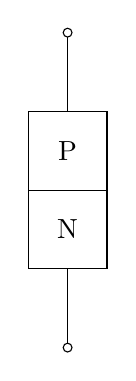
\begin{tikzpicture}
            \draw (0,2) to[short,o-] (0,1);
            \draw (0,-2) to[short,o-] (0,-1);
            \draw (-0.5,1) rectangle (0.5,-1);
            \draw (-0.5,0) to (0.5,0);
            \node at (0,0.5) {P};
            \node at (0,-0.5) {N};
        \end{tikzpicture}
        \qquad\qquad\qquad
        \begin{tikzpicture}
            \draw (0,2) to[diode,o-o] (0,-2);
            \draw[-stealth] (1,0.5) to (1,-0.5);
            \node[right] at (1,0) {$v_D,i_D$};
        \end{tikzpicture}
    \end{center}
    \par PN结二极管有一个势垒电压,取$0.7\mathrm{V}$。当$v_D<0.7\mathrm{V}$时,此时的电流极其微小,只有$\mathrm{fA}$
    量级,降低电压不会引起电流的明显变化,达到\textbf{电流饱和},一般取饱和电流$I_{S0}=1\mathrm{fA}$。当$v_D>0.7\mathrm{V}$时,$i_D$满足
    \[
    i_D=I_{S0}(e^{\frac{v_D}{v_T}}-1)    
    \]
    \par 其中
    \[
    v_T=\frac{kT}{q}\approx 26\mathrm{mV}\quad(298\mathrm{K})    
    \]
    $k$是玻尔兹曼常数,$T$是温度,$q$是电荷量,这里是电子的电量。在室温($25^\circ \mathrm{C}\approx298\mathrm{K}$)
    下取值为$26\mathrm{mV}$。
    \par 一般二极管应该避免被击穿,而Zener二极管则专门设计工作在反向击穿区。反向击穿区有三个重要的工作点:(1)拐点电流
    $I_{ZK}$,反偏电流大于这个值才会进入击穿区;(2)测试电流$I_{ZT}$,相对应测出电压$V_Z$,$V_Z@I_{ZT}$;(3)最大电流
    $I_{ZM}$,二极管电流不应该超过这个值,否则有可能损毁二极管。
    \subsection{二极管的模型}
    \subsection{二极管的应用}

    \section{MOSFET及其应用}
    \section{BJT及其应用}




























\end{document}